The purpose of this chapter is to provide a quantifiable assessment of the persistent radio wave energy in the near-Earth space environment due to lightning-generated Whistlers. The morphology of LEP (time evolution, spatial extent at the Earth's surface, and so forth) are primarily determined by the location of wave-particle interactions; additionally, wave-particle interactions with Whistlers are hypothesized to be the primary cause of slot-region electron depletions, and the ``impenetrable barrier'' below L $\sim$ 2.

Lightning-generated Whistlers are sporadic, and exist alongside a multitude of radio wave activity, such as VLF chorus and plasmaspheric hiss, making a correlated \emph{in-situ} measurement challenging. Within this chapter we simulate the relative VLF energy (L-shell, latitude, longitude) in the near-Earth space environment, in volumetric units [J/$m^3$], as a means of assessing their relative contribution to the persistent radio spectrum.

%\section{Overview of Previous Work}

\section{Methodology}
Our simulation is divided into two portions: First, a simulation of persistent VLF energy due to a single flash originating at a fixed latitude, and second, an integration over a measured lightning dataset, using scaled and shifted ``stencils'' for each flash.

Figure \ref{fig:power_blockdiagram} shows the steps required to compute a single stencil. 
\begin{enumerate}
\item{First we model the sub-ionosphere power spectrum generated from a flash with a known peak current, using the methodology of section \ref{section:input_power}.}
\item{We then propagate the energies through the ionosphere, using the attenuating slab approximation method of section \ref{section:trans_ionosphere_atten}.}
\item{We map the effective power above the ionosphere (J/$m^2$ at 1000 km altitude) to an energy density along a fixed grid using a set of pre-computed ``guide rays" using the methodology in section \ref{section:raytracing}, the Landau damping from section \ref{section:damping}, and the novel interpolation scheme described below.}
\item{In order to account for multiple crossings at each grid point, and to reduce our output space across different latitudes, we store the time-averaged energy density along each field line.}
 \end{enumerate}
\begin{figure}
\begin{center}
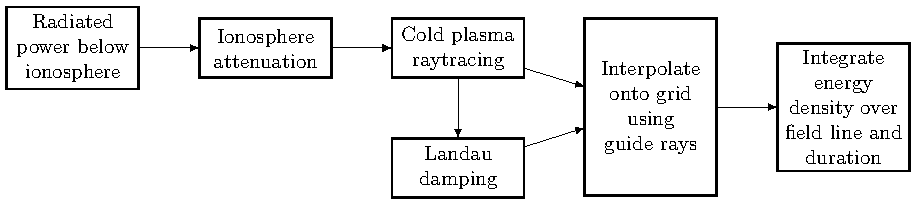
\includegraphics[width=\textwidth]{figures/lightning_power_block_diagram.pdf}
\caption[Energy density calculation block diagram]{Block diagram of the average energy density calculation for a single flash.}
\label{fig:power_blockdiagram}
\end{center}
\end{figure}

\section{Persistent Energy from a Single Flash}

\begin{table}
\caption{Simulation Parameters}
\begin{center}
\begin{tabular}{c|c}
Latitude spacing & 1$^\circ$ \\
Longitude spacing & 1$^\circ$ \\
Frequency range & 200 Hz - 30 kHz \\
Coarse Frequencies & 33 (log-spaced) \\
Fine Frequencies & 20 \\
\end{tabular}
\end{center}
\label{default}
\end{table}%

\subsection{Radiated power above the ionosphere}

% Illumination pattern
\begin{figure}
\begin{center}
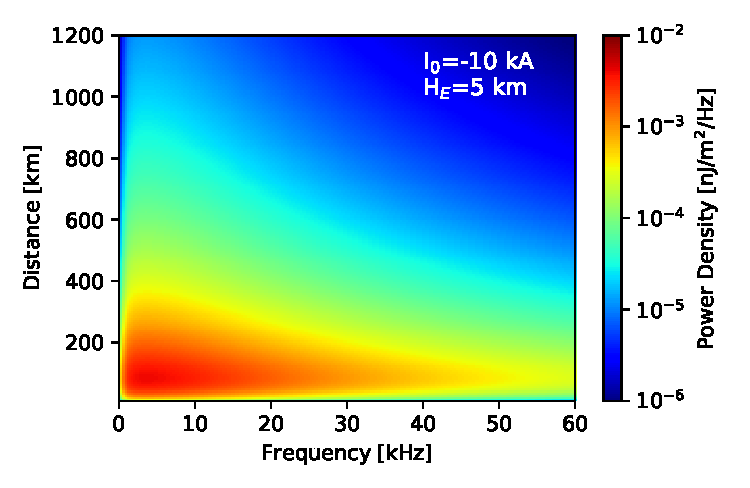
\includegraphics{figures/power_scaling_below_ionosphere.pdf}
\caption[Illumination pattern below the ionosphere]{Vertically-propagating power density from a single discharge, as a function of frequency and radial distance. Adapted from \cite{Marshall2011}.}
\label{fig:illumination}
\end{center}
\end{figure}


% Illumination pattern
\begin{figure}
\begin{center}
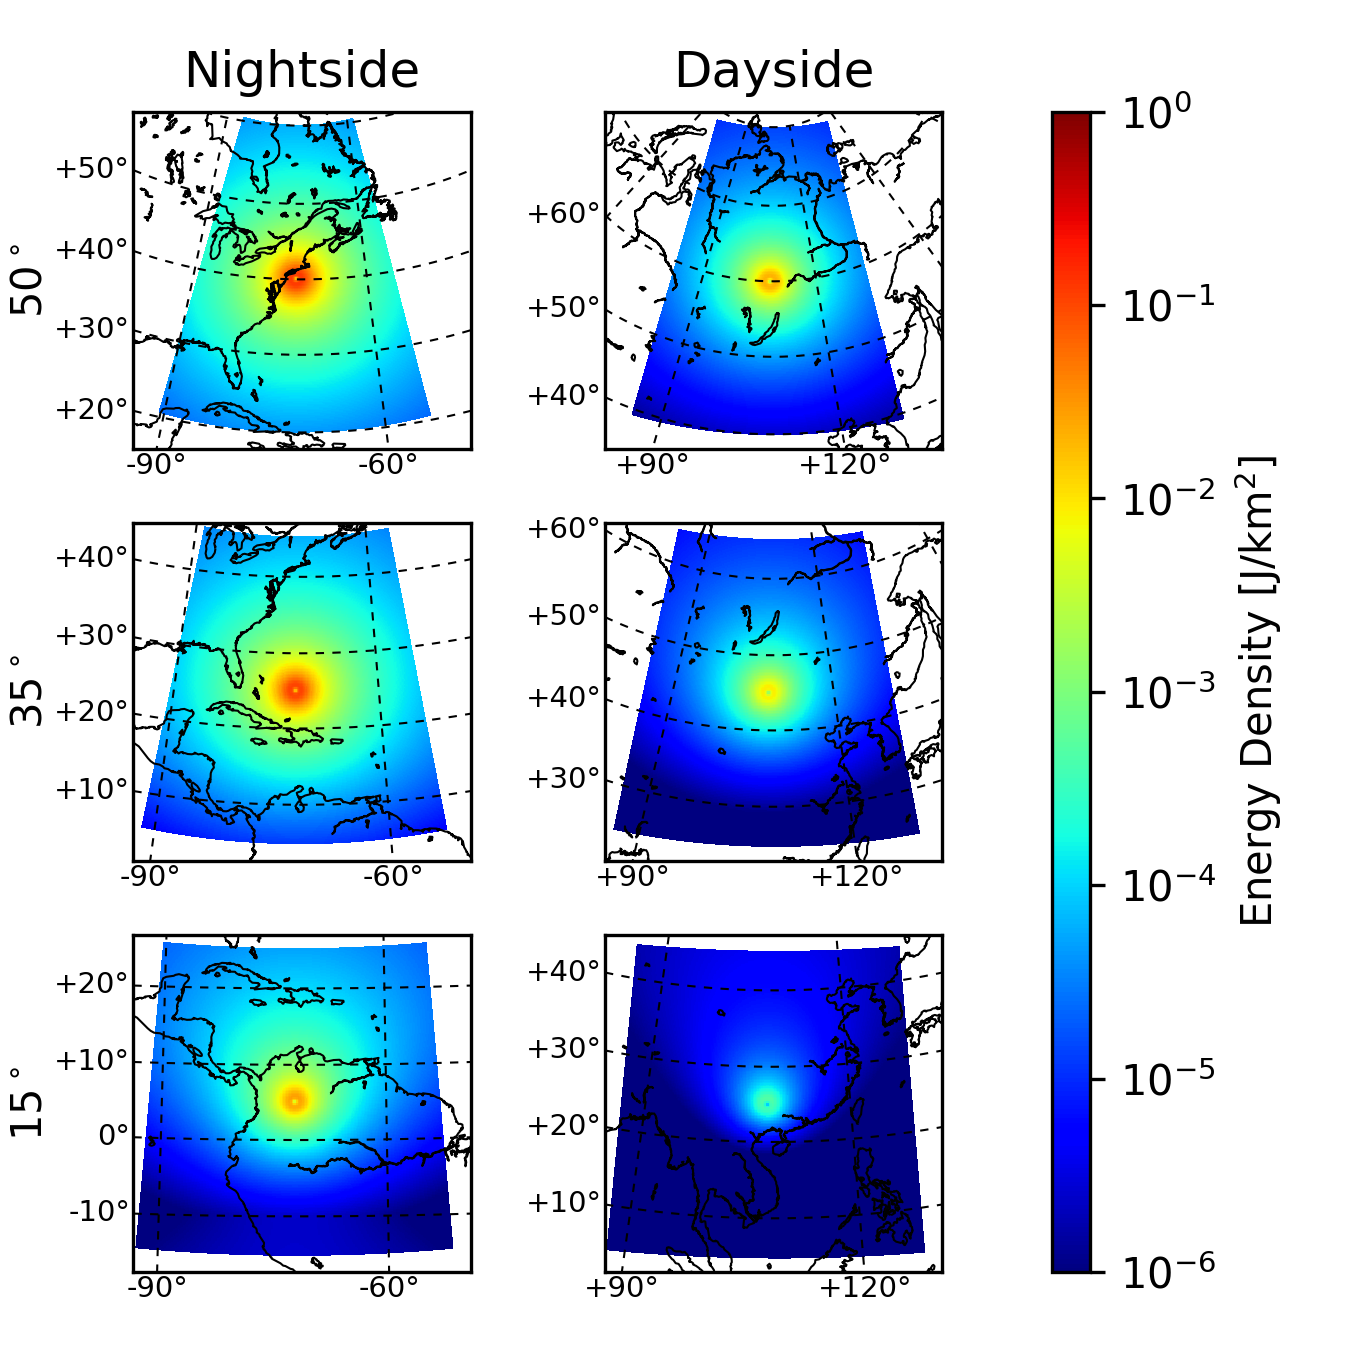
\includegraphics{figures/illumination_basemap.png}
\caption[Illumination pattern above the ionosphere]{Illumination pattern, integrated over frequency, after ionospheric attenuation (altitude = 1000 km).}
\label{fig:illumination}
\end{center}
\end{figure}

% Total energy above ionosphere
\begin{figure}
\begin{center}
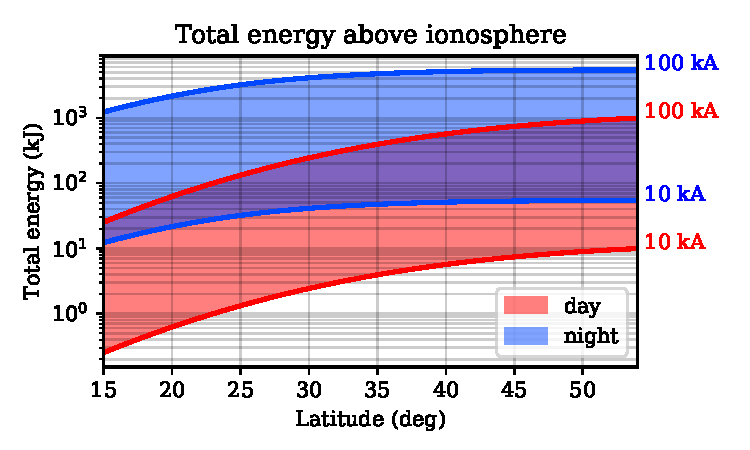
\includegraphics{figures/total_energy.pdf}
\caption[Energy above the ionosphere due to a single flash]{Integrated energy above the ionosphere from a single discharge, as a function of geomagnetic latitude. Energy scales quadratically with peak current; totals for 10 kA (an average flash), and 100 kA (a strong, but not unreasonable flash) are overlaid. }
\label{fig:illumination}
\end{center}
\end{figure}


\subsection{Gridding and Interpolation}

    \begin{figure}
    \centering
    \begin{subfigure}[t]{0.45\textwidth}
    \centering
        	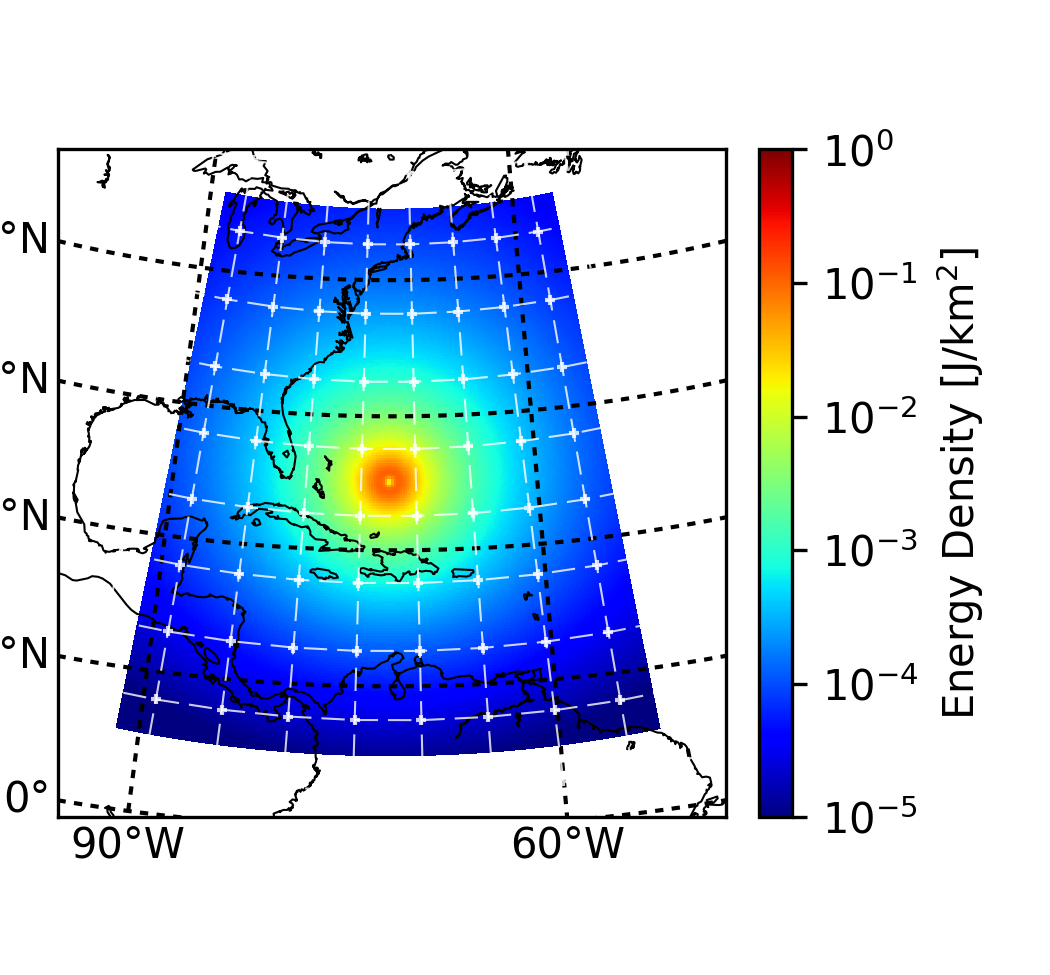
\includegraphics{figures/input_energy_with_grid.png}
	\caption{Input energy gridding}
        \label{fig:input_energy_grid}
    \end{subfigure}\hfill
    \begin{subfigure}[t]{0.45\textwidth}
    \centering
        	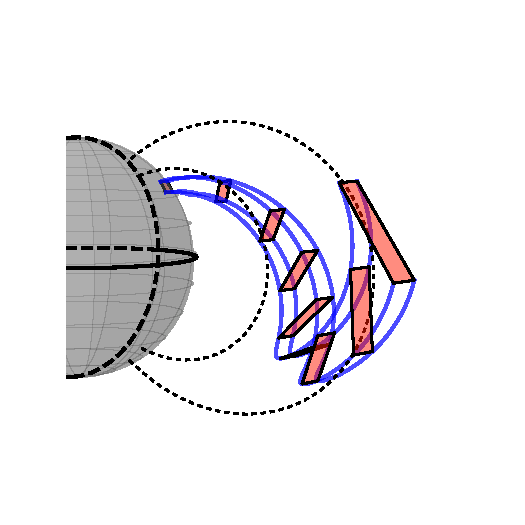
\includegraphics[trim={1cm 0.25cm 1cm 1cm},clip]{figures/interpolation_globe1.pdf}
	\caption{``guide ray'' construction}
        \label{fig:guide_rays}
    \end{subfigure}
    \caption{An illustration of the interpolation scheme. (a) Energy at the top of the ionosphere is divided into cells, in latitude, longitude, and frequency. Shown here with 5$^\circ$ cells (much larger than used in simulation). The plotted energy is integrated over frequency. (b) Illustration of the guide ray method. Input energy is integrated between a set of guide rays, spaced in latitude, longitude, and frequency. This energy is then averaged over a 4-dimensional volume, bounded by two adjacent timesteps $t-1$, $t$ of the guide rays.}
    \label{fig:interpolation_scheme}
\end{figure}


% Delaunay figure
\begin{figure}
\begin{center}
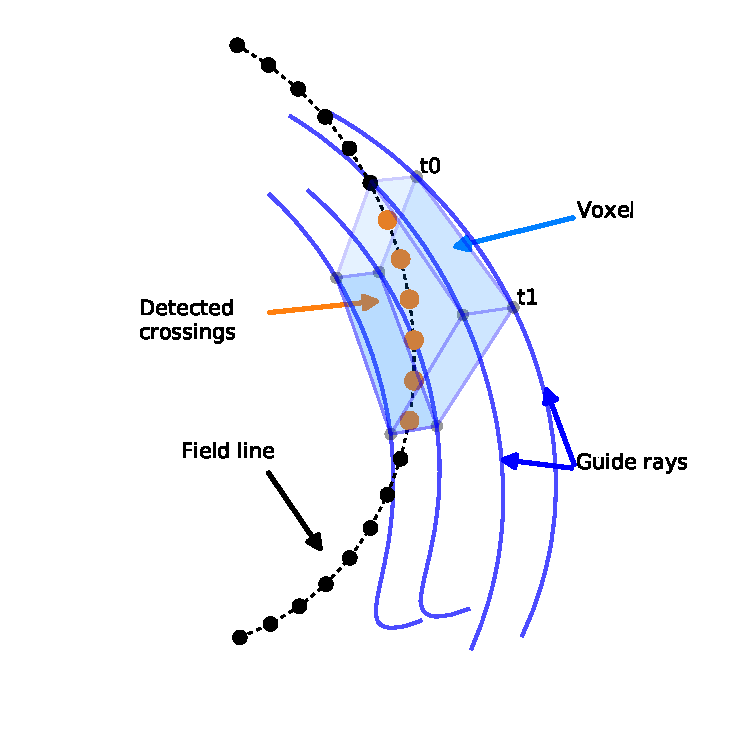
\includegraphics{figures/delaunay_1.pdf}
\caption{Illustration of the Delaunay interpolation method, shown here in three dimensions (e.g., for a single frequency).}
\label{fig:delaunay_1}
\end{center}
\end{figure}

% Fine-scale frequency interpolation
\begin{figure}
\begin{center}
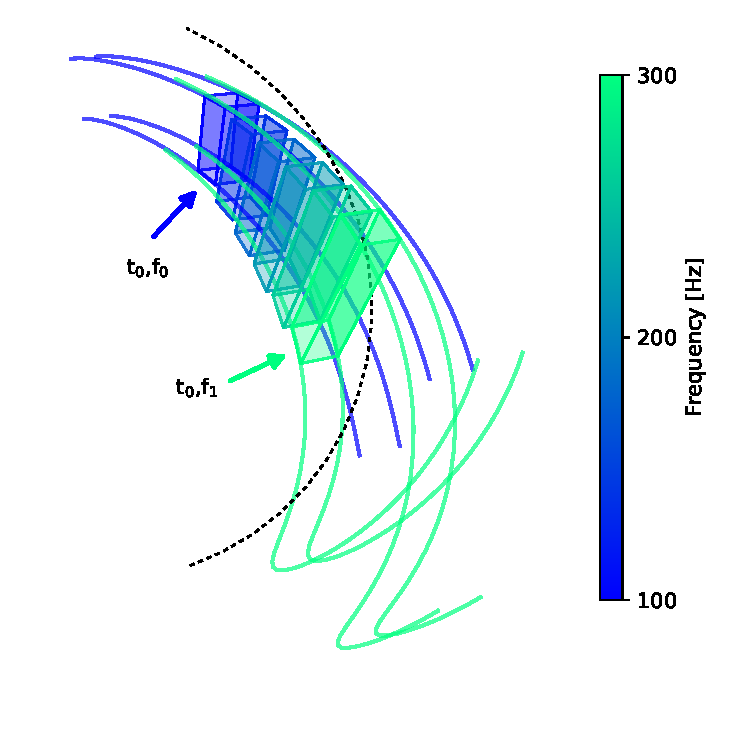
\includegraphics{figures/delaunay_2.pdf}
\caption{Fine-scale frequency interpolation.}
\label{fig:delaunay_2}
\end{center}
\end{figure}

% CONVEX HULL FIGURE
\begin{figure}
\begin{center}
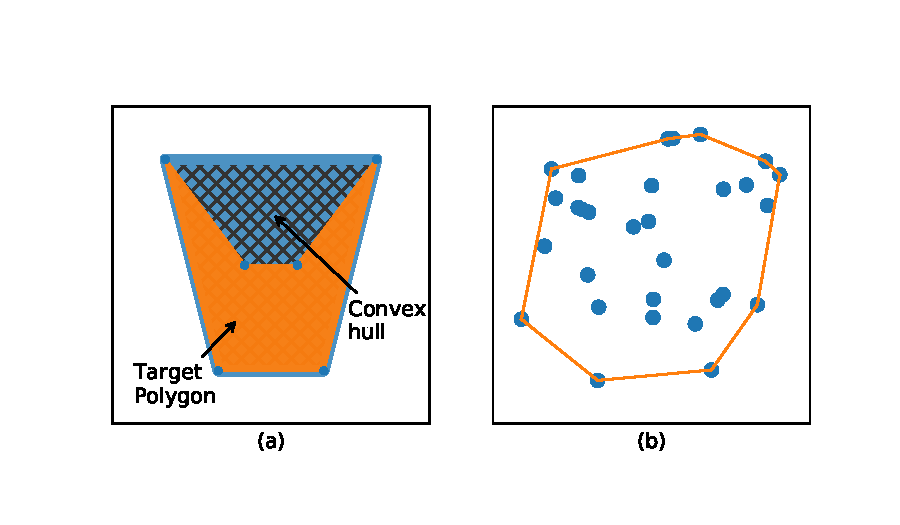
\includegraphics{figures/convex_hulls.pdf}
\caption{Illustration of a convex hull in two dimensions.}
\label{fig:convex_hulls}
\end{center}
\end{figure}



\begin{figure}
\begin{center}
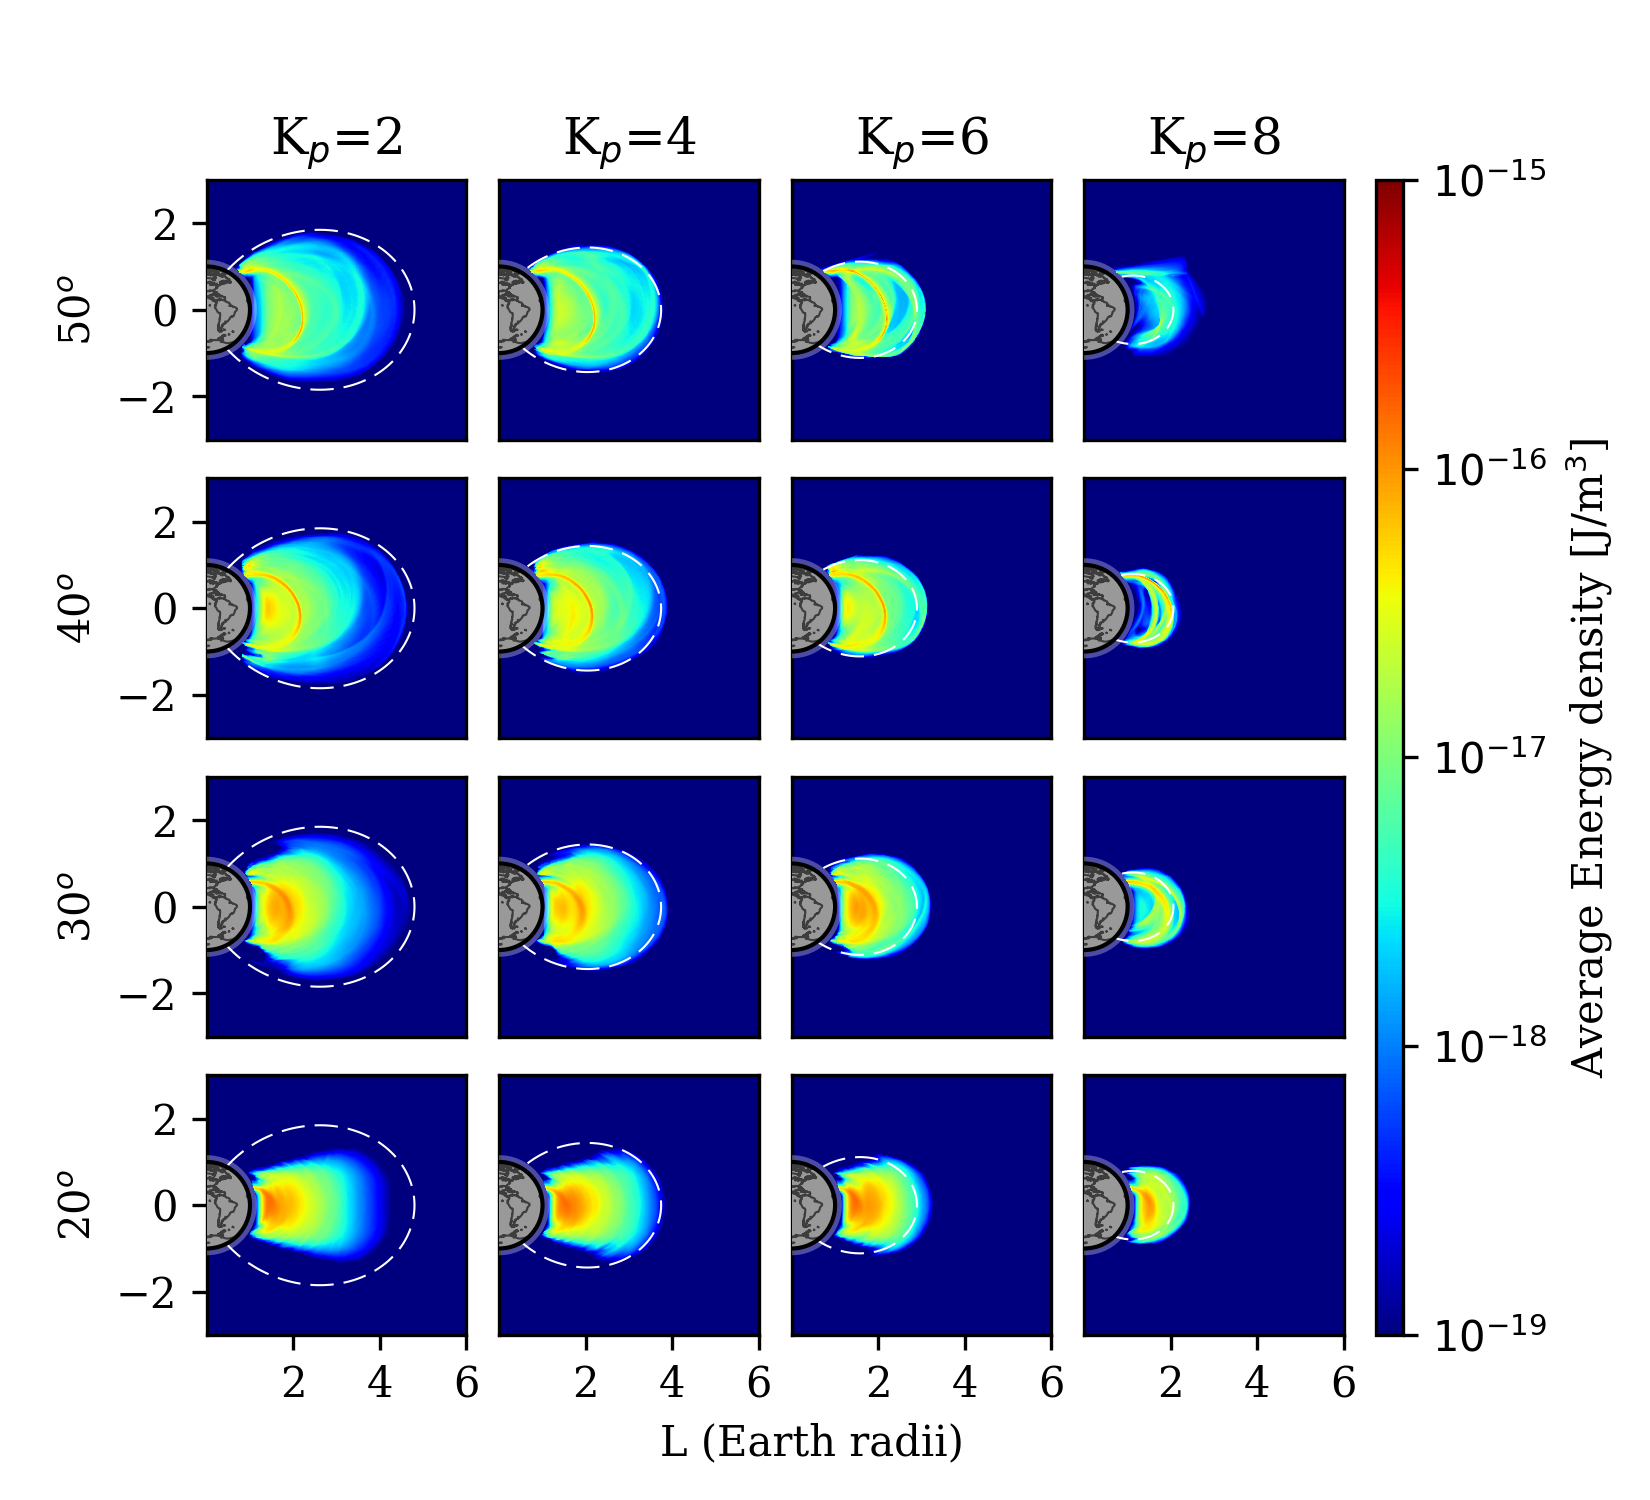
\includegraphics[draft]{figures/energy_from_single_flash_meridonal_plane.pdf}
\caption{Block diagram}
\label{fig:energy_from_single_flash}
\end{center}
\end{figure}

% you'll want to put a figure showing the volume averaging too...

\begin{figure}
\begin{center}
\includegraphics[draft]{figures/energy_in_meridional_plane_movieframes.pdf}
\caption{Block diagram}
\label{fig:energy_from_single_flash}
\end{center}
\end{figure}


\begin{figure}[ht]
\begin{center}
\includegraphics[draft]{figures/energy_stencils.pdf}
\caption{Block diagram}
\label{fig:energy_stencils}
\end{center}
\end{figure}

\section{Global Energy Density}

\begin{figure}
\begin{center}
\includegraphics[draft]{figures/energy_density_vs_L_vs_freq.pdf}
\caption[Average energy density vs L and frequency]{Average energy density as a function of L-shell and wave frequency}
\label{fig:energy_density_vs_L_vs_freq}
\end{center}
\end{figure}
